
\begin{figure}[h]
    \centering

    \advance\leftskip-3.5cm
    \advance\rightskip-4cm
	
	\minipage{0.30\textwidth}
	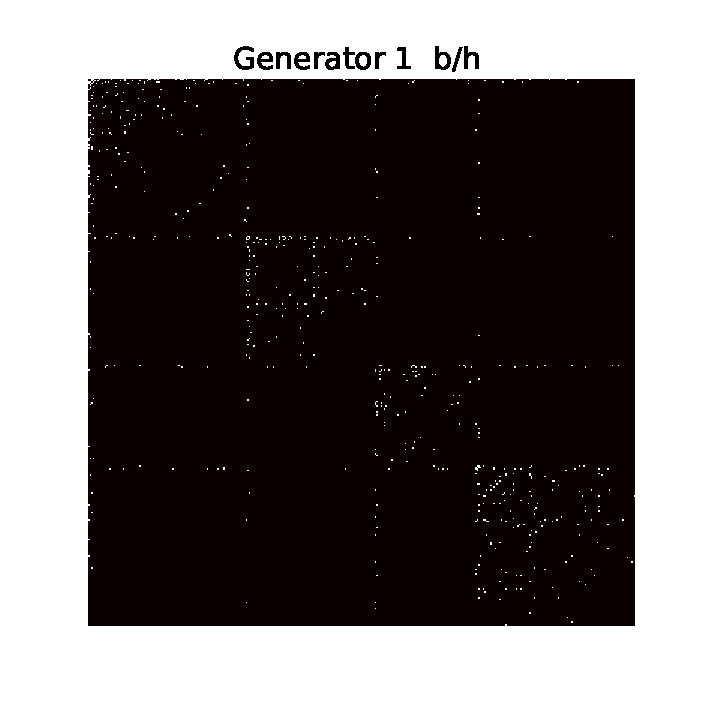
\includegraphics[scale=0.32]{img/g1}
	\endminipage
	\minipage{0.30\textwidth}
	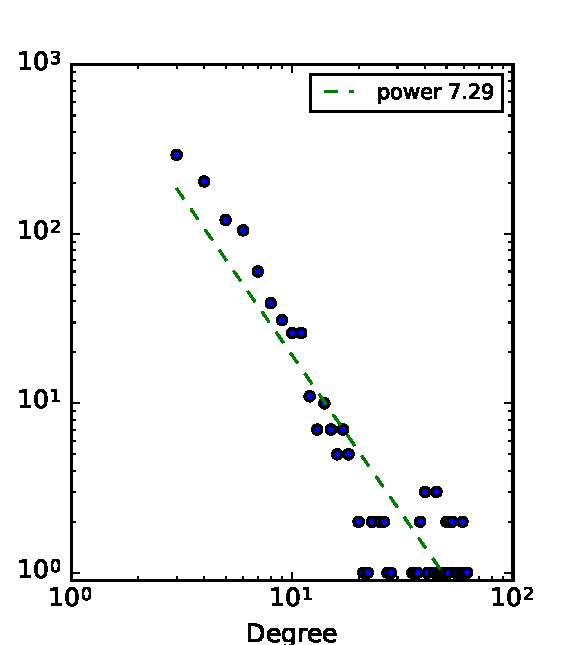
\includegraphics[scale=0.32]{img/g1_d}
	\endminipage
	\vspace{-0.4cm}
	\minipage{0.30\textwidth}
	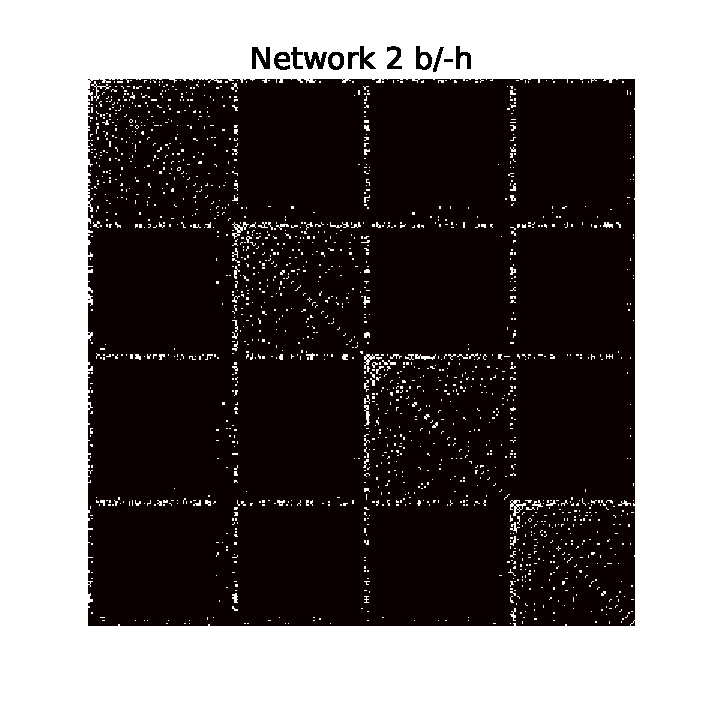
\includegraphics[scale=0.32]{img/g2}
	\endminipage
	\minipage{0.30\textwidth}
	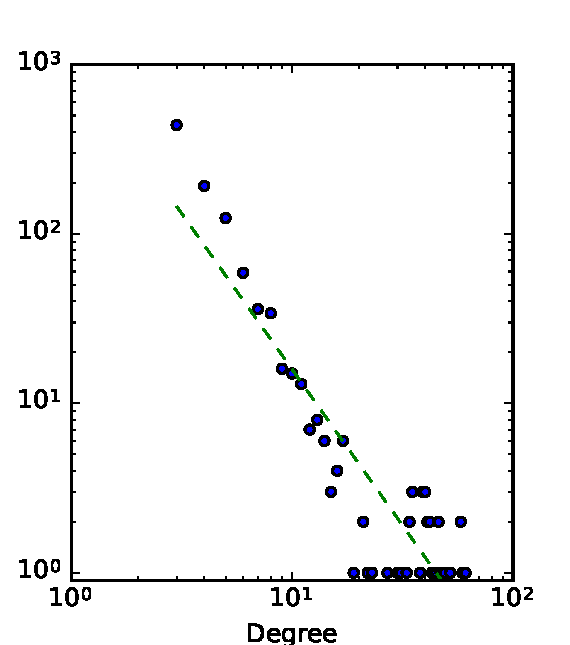
\includegraphics[scale=0.32]{img/g2_d}
	\endminipage

	%\vspace{-0.4cm}

	\minipage{0.30\textwidth}
	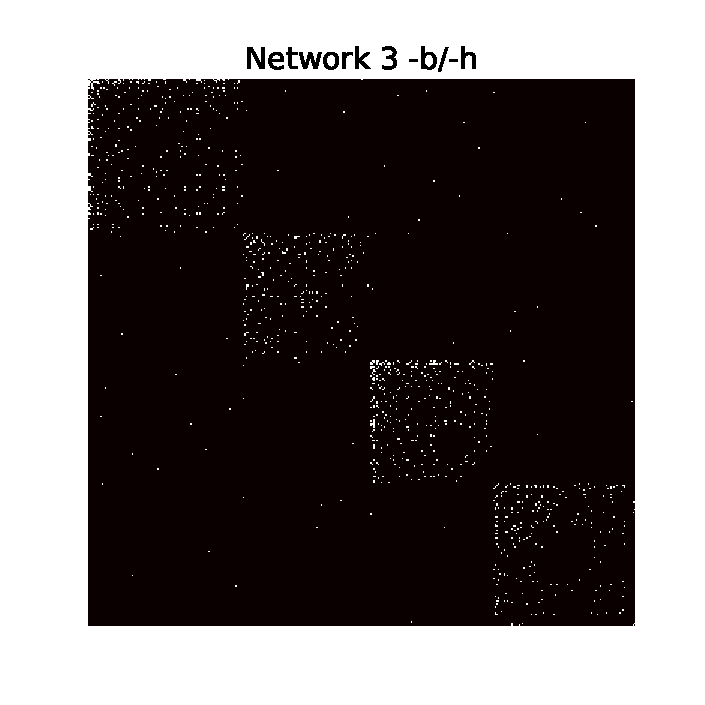
\includegraphics[scale=0.32]{img/g3}
	\endminipage
	\minipage{0.30\textwidth}
	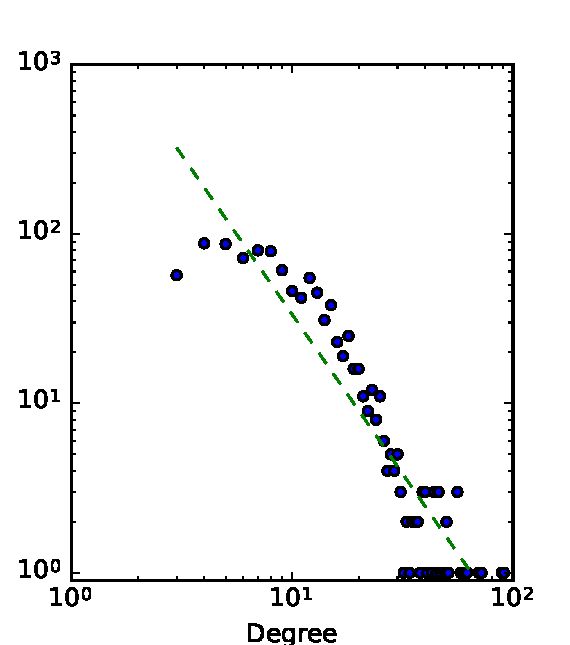
\includegraphics[scale=0.32]{img/g3_d}
	\endminipage
	\vspace{-0.4cm}
	\minipage{0.30\textwidth}
	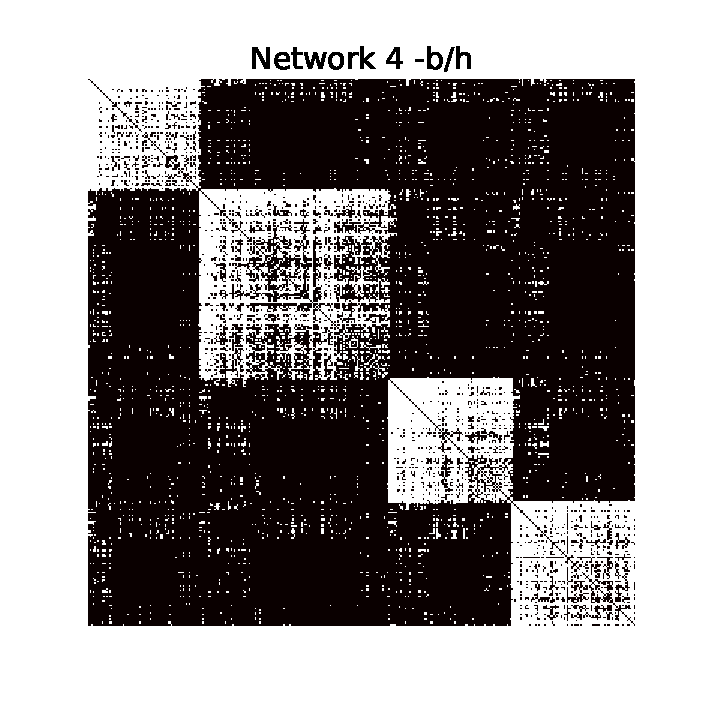
\includegraphics[scale=0.32]{img/g4}
	\endminipage
	\minipage{0.30\textwidth}
	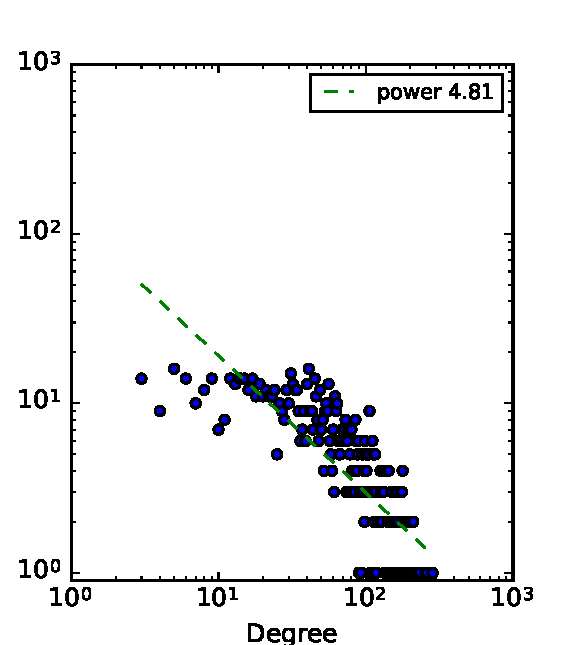
\includegraphics[scale=0.32]{img/g4_d}
	\endminipage
	
	\caption{Left subfigures represent the adjacency matrices for each of the 4 synthetic networks that we used for the prediction evaluation along with theirs respective global degree distribution in the right subplots.}
	\label{fig:synt_graph}
\end{figure}

\vspace{1cm}
